\chapter{Ants}
\label{sec:module.Ants}

Alle Klassen im Ants Package sind spezifisch f�r die Ants AI Challenge und machen das Ger�st unseres \gls{Bot}s aus. Nachfolgend wird deren Aufbau erl�utert.

\section{State-Klassen}
\label{sec:module.Ants.State}

\begin{figure}[H]
\centering
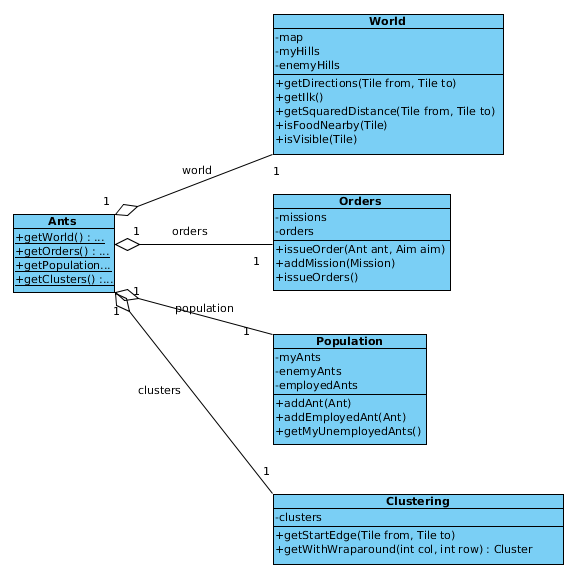
\includegraphics[width=0.7\textwidth]{91_bilder/State}
\caption{State-Klassen}
\label{fig:StateClasses}
\end{figure}

Abbildung \ref{fig:StateClasses} zeigt eine \"{U}bersicht der Spielzustands-Klassen. F�r das Diagramm wurden lediglich die wichtigsten Methoden und Attribute ber�cksichtigt. Die State-Klassen implementieren alle das Singleton-Pattern.

\subsection{Ants}
\label{sec:module.Ants.State.Ants}
Die Ants Klasse ist die zentrale State-Klasse. Sie bietet einfachen Zugriff auf die anderen State-Klassen. Urspr�nglich hatten wir alle Methoden, die mit dem Zugriff auf den Spielzustand zu tun hatten, direkt in der Ants Klasse implementiert, haben aber schnell gemerkt, dass das unhandlich wird und haben die Zust�nde in die Klassen World, Population und Orders aufgeteilt. Die Ants Klasse dient jetzt vor allem als Container f�r die anderen State-Klassen und implementiert nur noch einige Methoden, die Zustands�nderungen in verschiedenen Bereichen vornehmen.

\subsection{World}
\label{sec:module.Ants.State.World}
Die World Klasse enth�lt Informationen zur Spielwelt und erweitert die AbstractWrapAroundMap aus der AI-Tools API. Hier wird die Karte abgespeichert, in der f�r jede Zelle die aktuell bekannten Informationen festgehalten werden. Das beinhaltet die Sichtbarkeit der Zelle und was die Zelle aktuell enth�lt (Ameise, Nahrung, Wasser, ...). Ausserdem werden Listen gef�hrt, wo sich die eigenen und die bekannten gegnerischen H�gel befinden. Die Klasse bietet Methoden zur Distanzberechnung und gibt Auskunft �ber einzelne Zellen, beispielsweise ob sich Nahrung in der Umgebung einer bestimmten Zelle befindet. Zudem sind die wichtigsten Methoden des SearchableMap Interfaces (\texttt{getSuccessors...()}) hier implementiert.

\subsection{Orders}
\label{sec:module.Ants.State.Orders}
In der Orders Klasse wird �ber Befehle und Missionen der einzelnen Ameisen Buch gef�hrt. In der Liste der Befehle wird zwischengespeichert, welche Ameise welche Bewegung im aktuellen Spielzug macht. Zu Beginn des Spielzuges wird diese geleert, dann von den Tasks und Missionen mit Befehlen belegt, und am Schluss des Spielzuges werden die Befehle der Spielschnittstelle �bergeben. Die Liste der Missionen ist zug�bergreifend gef�hrt, da eine Mission �ber mehrere Spielz�ge verlaufen kann. Das zentrale Verwalten der Befehle und Missionen dient dazu, sicherzustellen, dass keine widerspr�chlichen Befehle ausgegeben werden wie: Mehrere Befehle f�r eine Ameise, gleiche Ziel-Koordinaten f�r mehrere Ameisen, eine Ameise ist mehreren Missionen zugeteilt etc..

\subsection{Population}
\label{sec:module.Ants.State.Population}
Die Population Klasse dient der Verwaltung der eigenen und der gegnerischen Ameisen-V�lker. Hier werden die Ameisen mit ihren aktuellen Aufenthaltsorten festgehalten. Wenn f�r eine Ameise ein Befehl ausgegeben wird, wird die Ameise als besch�ftigt markiert. \"{U}ber die Methode \texttt{getMyUnemployedAnts()} kann jederzeit eine Liste der Ameisen abgefragt werden, die f�r den aktuellen Zug noch keine Befehle erhalten haben und f�r neue Aufgaben zur Verf�gung stehen. Die Population Klasse f�hrt zudem Buch �ber die verf�gbaren Ressourcen pro Aufgabentyp und stellt sicher, dass kein Aufgabentyp mehr Ressourcen beansprucht, als ihm zugeteilt sind. (s. Kapitel \ref{sec:module.resourceMgmt})


\section{Spiel-Elemente (Ants-Spezifisch)}
\label{sec:module.Ants.State.Entities.Ants}

\begin{figure}[H]
\centering
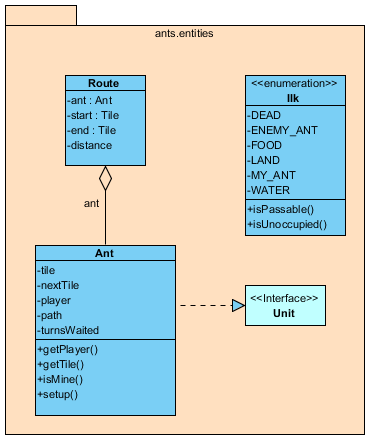
\includegraphics[width=0.5\textwidth]{91_bilder/antsEntities}
\caption{Ants-spezifische Elemente der Spielwelt}
\label{fig:antsEntities}
\end{figure}

Abbildung \ref{fig:antsEntities} zeigt die wichtigsten Klassen, die die Elemente des Spiels repr�sentieren. Der \"Ubersichtlichkeit wegen wurden nur die wichtigsten Attribute und Operationen in das Diagramm aufgenommen.

\subsection{Ant}
\label{sec:implementation.Entities.Ant}
Eine Ant (Ameise) geh�rt immer zu einem Spieler; �ber die Methode \texttt{isMine()} k�nnen unsere eigenen Ameisen identifiziert werden. 
Die Ant Klasse implementiert das Interface Unit aus der AITools-API, welches eine Abstraktion bietet, die die Verwendung der Ameisen in den generischen Modulen erlaubt.
Eine Ameise weiss jeweils, in welcher Zelle sie steht. Das Feld \texttt{nextTile} dient der Verfolgung einer Ameise �ber mehrere Z�ge. Der Wert des Felds wird jeweils gesetzt, wenn der Ameise ein n�chster Zug zugewiesen wird. Im n�chsten Spielzug wird die Position der Ameise durch diese Information aktualisiert.

\subsection{Route}
\label{sec:implementation.Entities.Route}
Eine Route repr�sentiert eine einfache Verbindung zwischen zwei \gls{Tile}s. Die Distanz zwischen den \gls{Tile}s wird mit der Luftliniendistanz gemessen.

\subsection{Ilk}
\label{sec:implementation.Entities.Ilk}
Ilk ist der Typ einer Spielfeldzelle. Der Ilk einer \gls{Tile}-Instanz gibt an, was sich gerade in der Zelle befindet. Dies kann ein Gel�ndetyp sein, wenn die Zelle nicht besetzt ist, oder es kann eine Ameise, Nahrung, oder ein H�gel sein; in diesem Fall ist der Gel�ndetyp implizit ''Land``, da Wasser-\gls{Tile}s nicht besetzt sein k�nnen. Die Ilk-Enumeration bietet Hilfsmethoden, um festzustellen, ob eine Zelle passierbar oder besetzt ist.
